\documentclass[10pt]{beamer}
\usetheme{Malmoe}
\setbeamertemplate{navigation symbols}{}
%\colorlet{beamer@blendedblue}{blue!40!black}
\setbeamertemplate{navigation symbols}{}
\newcommand*\oldmacro{}%
\let\oldmacro\insertshorttitle%
\renewcommand*\insertshorttitle{%
\oldmacro\hfill%
\insertframenumber\,/\,\inserttotalframenumber}

\usepackage{caption}
\usepackage{hyperref}
\usepackage[makeroom]{cancel}
\usepackage{ amssymb }
\usepackage{appendixnumberbeamer}
%\usepackage{tikz-feynman}
\usepackage{graphicx}
\begin{document}

\title{Nationwide: Model Risk Management Assessment/Case Study}
\author[Barkeloo]{Jason Barkeloo, Ph.D.}
\date{November 16, 2020}

%\titlegraphic{\includegraphics[width=4cm]{../ATLAS-Logo-Ref-RGB.png}\hspace*{2.75cm}~%
%   \includegraphics[width=4cm]{../uo_logo_green_on_white_2.jpg}
%}

\frame{\titlepage}
\frame{\frametitle{Table of Contents}\tableofcontents[hidesubsections]}

\frame{\frametitle{Code location for further fleshed out examples}

All code for these exercises can be found via this hyperlink as a ipython/jupyter notebook located on my github in addition to attachments sent with the presentation: \\~\\


\hyperlink{https://github.com/JTBarkeloo/JupyterNotebooks/blob/master/MRM Assessment.ipynb}{https://github.com/JTBarkeloo/JupyterNotebooks/blob/master/MRM Assessment.ipynb} 

}

\section{Exploratory Analysis}

\frame{\frametitle{Exploratory Data Analysis}
Summary of 30,000 individuals
\begin{itemize}
\item age - Age of customer
\item inc - Income of customer
\item car - Category of car: Standard, Luxury, Truck
\item edu - Education level of driver (High School or College)
\item acc - Number of accidents over the last two years

\end{itemize}
Want to build a model that will optimize recognition of accident events using these values and attempt to categorize riskier drivers from less risky drivers
Ideal model would have nice bifurcation between classes, difficult to get without more discriminating variables with separation power

%\centering
%\includegraphics[width=0.7\textwidth]{../../ThesisImages/backgrounds.png}
}

\frame{\frametitle{Exploratory Data Analysis}
\begin{itemize}
\item Start by looking at behavior of noncategorical data, Age is oddly uniform
\end{itemize}
\centering
\begin{columns}
\begin{column}{0.5\textwidth}
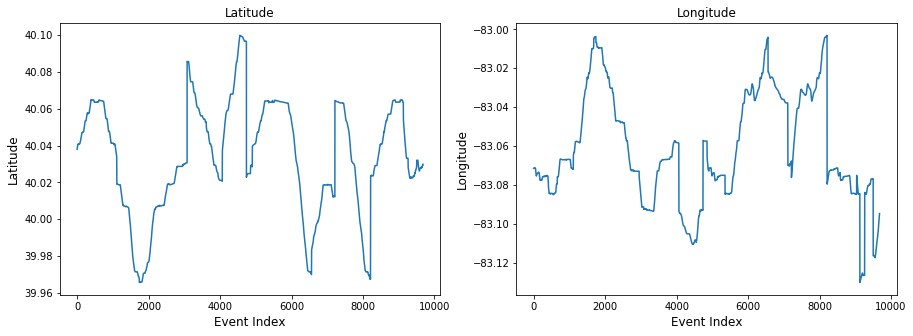
\includegraphics[width=0.9\textwidth]{Images/Image2.png}
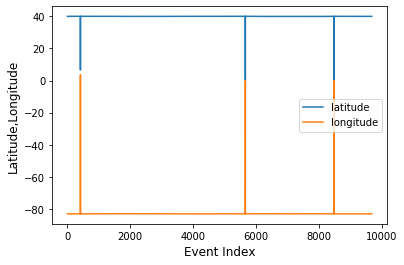
\includegraphics[width=0.9\textwidth]{Images/Image1.png}
\end{column}
\begin{column}{0.5\textwidth}
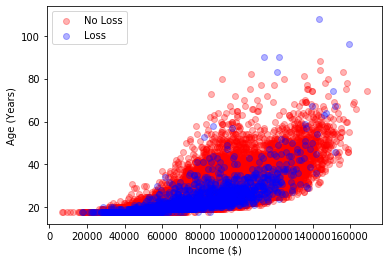
\includegraphics[width=0.9\textwidth]{Images/Image5.png}
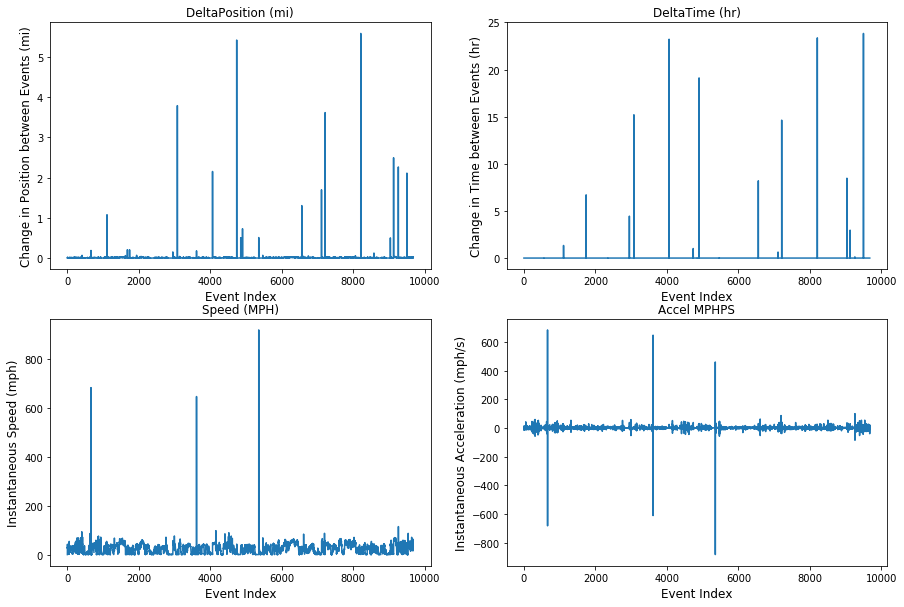
\includegraphics[width=0.9\textwidth]{Images/Image3.png}
\end{column}
\end{columns}
}

%\frame{\frametitle{Further Cleaning - $\Delta$Position, $\Delta$Time, Speed, Acceleration}
%\centering
%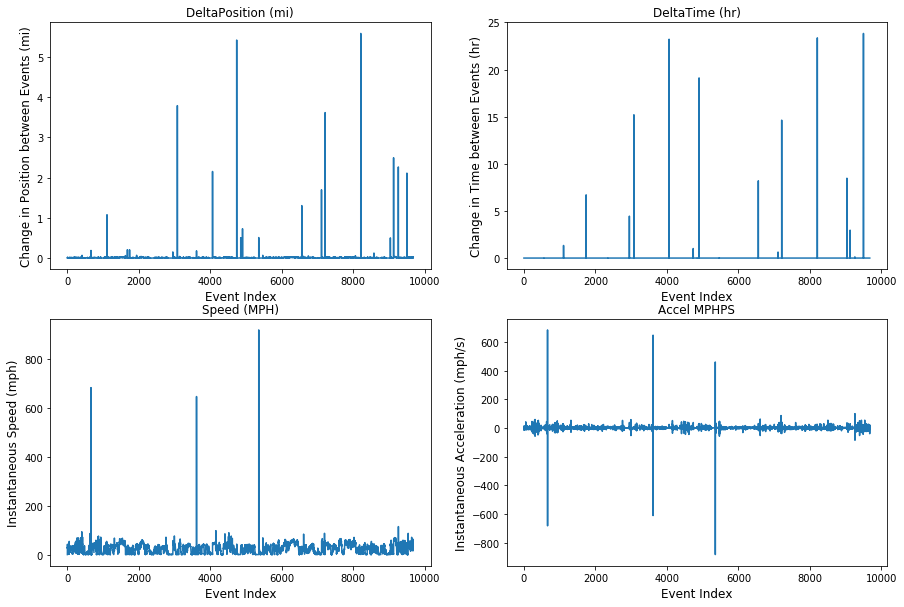
\includegraphics[width=1.\textwidth]{Images/Image3.png}
%}



%%%%%%%%%%%%%%%%%%%%%%%%%%%%%%%%%%%%%%%%%%%%%%%%%%%%%%%%%%%%%%%%%



\frame{\frametitle{Statistical Significance: Vehicle and Education Types}
Z-test used, conclusions to be drawn depend on how liberal the definition of statistical significance being used is \\ 
The use of p$<$0.05 is somewhat arbitrary but is what will be used here as it is a standard choice of convention
\begin{itemize}
\item z value for Standard and Luxury: 3.64
\item z value for Standard and SUV: 5.31 
\item z value for Luxury and Truck: 7.11 
\end{itemize}
The null hypothesis can be rejected for all combinations of Vehicle Types \\
\begin{itemize}
\item z value for High School and College: 0.27
\end{itemize}
The null hypothesis cannot be rejected for Education Types, as such for my models they will be combined and education type not used as a potential discriminator \\~\\
Categorical variables are changed to numbers using one-hot encoding to prevent ranking errors during model building and testing.
}




%%%%%%%%%%%%%%%%%%%%%%%%%%%%%%%%%%%%%%%%%%%%%%%%%%%%%%%%%%%%%%%%%%
\section{Model Building}

\frame{\frametitle{Model Building}
A variety of models were employeed to different ends to try and create a binary classification of risk.  Multiple collision events are classified with single collision events.  With more data a third category of excessive risk could be added to models.  \\~\\
Small minority class, small percentage of those are multiple collision events. \\~\\
Models presented here (with smote oversampling training data):
\begin{itemize}
\item Logistic Regression
\item Boosted Decision Tree (BDT) 
\end{itemize}
A training (80\%)/testing(20\%) random set split was done to help ensure unbiased results
%\centering
%\includegraphics[width=0.7\textwidth]{../../ThesisImages/backgrounds.png}
}

\frame{\frametitle{Multivariate Logistic Regression}
\begin{itemize}
\item Naively we could train a model on the data classes as given
\item With enough separation power i.e., variables distinct enough in each class, this can be used for event classification
\item SMOTE Oversampling used to generate synthetic data that is similar to, but not exactly like the minority class, using a nearest-neighbors approach and fills in space between neighbors
\item Balanced Accuracy score: 0.559, Loss Event Accuracy: 0.575
\end{itemize}
\begin{columns}
\begin{column}{0.5\textwidth}
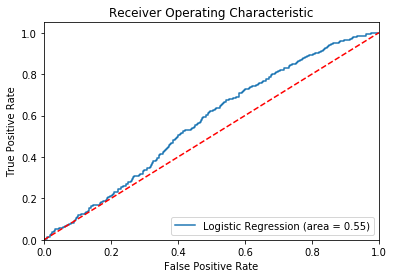
\includegraphics[width=0.9\textwidth]{Images/Image6.png}
\end{column}
\begin{column}{0.5\textwidth}
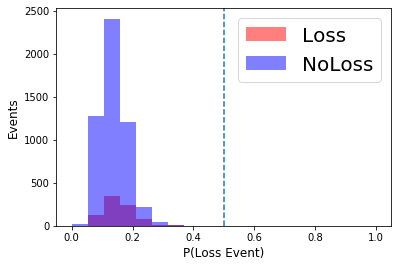
\includegraphics[width=0.9\textwidth]{Images/Image12.png}
\end{column}
\end{columns}
}

\frame{\frametitle{BDT with SMOTE Upsampling}
\begin{itemize}
\item A BDT was created and trained using SMOTE over-sampling with similar results
\item F Scores can give insight into separation powers of training variables
\item Weight: How frequent splitting occurs on the variable
\item Gain: How useful variable is in terms of separation
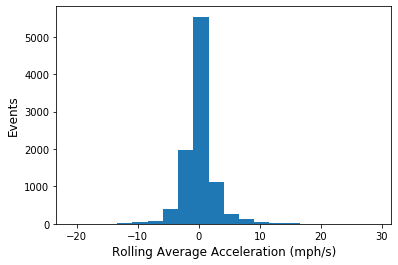
\includegraphics[width=0.9\textwidth]{Images/Image8.png}
\end{itemize}
\begin{columns}
\begin{column}{0.5\textwidth}
%\includegraphics[width=0.9\textwidth]{Images/Image15.png}
\end{column}
\begin{column}{0.5\textwidth}
%\includegraphics[width=0.9\textwidth]{Images/Image16.png}
\end{column}
\end{columns}
Loss Events P(Loss Event): mean: 0.510, std: 0.096 \\
NoLoss Events P(LossEvent): mean: 0.480, std: 0.097 \\
Loss Event Accuracy: 55.7\%
}

\frame{\frametitle{Model Comments}
\begin{itemize}
\item  Neural networks have been created and trained on a limited set of input variable with success in determination of Loss events
\item The addition of further independent input variables would help the separation of the neural network greatly
\item A bifurcation of the distributions is starting to occur with the ADASYN network, more input variables and events is likely to cause a major splitting of the distribution into likely Loss events and likely NoLoss events \\
%\item ADASYN over-sampling focuses on the decision boundary which leads to large flucuations in the validation accuracy
\item Boosted decision tree (BDT) models were also employed in the Jupyter notebook to slightly different ends
\end{itemize}
}

%\frame{\frametitle{}
%}

\section{Model Assessment}

\subsection{Model Limitations}
\frame{\frametitle{Title}
Can Multiple Loss Models be Useful Based on Driver Class i.e., Rural Vs. Urban Drivers?
\begin{itemize}
\item Rural and Urban drivers face different landscapes of challenges on their daily travels
\item Requirement: GPS definition of urban environments
\item Expect longer distance/trip for rural drivers while urban drivers have more stop-and-go traffic 
\item Larger Distances and a larger amount of HardAccelerations are both positvely correlated with loss this seems to be an interesting intersection of these correlations
\end{itemize}
\centering
%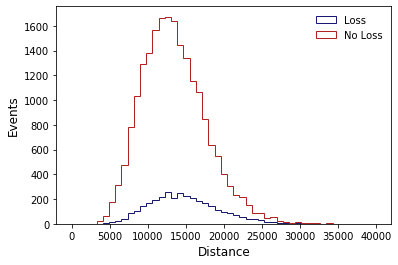
\includegraphics[width=0.4\textwidth]{Images/image18.png}
}

%\frame{\frametitle{Conclusion}
%\begin{itemize}
%\item Orthogonal validation/control regions are in development
%\end{itemize}
%}


%%%%%%%%%%%%%%%%%%%%%%%%%%%%%%%%%%%%%%%%%%%%%%%%%%%%%%%%%%%%%%%%
%%%%%%%%%%%%%%%%%%%%%%%%%%%%%%%%%%%%%%%%%%%%%%%%%%%%%%%%%%%%%%%% 	
%\appendix
%\section{Backup}
%\frame{\frametitle{Backup}
%}
\end{document}

%36.070
